\doublespacing
%% ------------------------------------------------------------------------- %%
\chapter{Aeross\'{o}is}
\label{cap:aerossois}

Os aeross\'{o}is atmosf\'{e}ricos s\~{a}o part\'{\i}culas min\'{u}sculas, l\'{\i}quidas ou s\'{o}lidas, que existem em suspens\~{a}o na atmosfera da Terra. Essas min\'{u}sculas part\'{\i}culas influenciam, sob v\'{a}rios aspectos, a vida na Terra: controlam a visibilidade no ar, a intensidade de radia\c{c}\~{a}o solar incidente e refletida pela superf\'{\i}cie da Terra, assim como as propriedades el\'{e}tricas e radiativas do meio ambiente. Os aeross\'{o}is atmosf\'{e}ricos tamb\'{e}m desempenham um papel fundamental na regula\c{c}\~{a}o do ciclo hidrol\'{o}gico da natureza, uma vez que got\'{\i}culas de \'{a}gua das nuvens s\~{a}o formadas pela condensa\c{c}\~{a}o do vapor de \'{a}gua da atmosfera na superf\'{\i}cie destes aeross\'{o}is.

Os aeross\'{o}is atmosf\'{e}ricos formadores de got\'{\i}culas de nuvens recebem o nome de n\'{u}cleos de condensa\c{c}\~{a}o de nuvens (CCN - Cloud Condensation Nuclei). \'{E} sabido que a estrutura das nuvens depende fortemente das caracter\'{\i}sticas desses n\'{u}cleos, os quais determinam a forma\c{c}\~{a}o de precipita\c{c}\~{a}o e a transfer\^{e}ncia, atrav\'{e}s das nuvens, da radia\c{c}\~{a}o solar incidente ou refletida pela Terra \cite{Mendes}.

Dependendo das naturezas f\'{\i}sica, qu\'{\i}mica e da quantidade de vapor na atmosfera, os CCNs podem iniciar o processo de forma\c{c}\~{a}o de got\'{\i}culas de nuvens \cite{HSU}. Assim sendo, as caracter\'{\i}sticas microf\'{\i}sicas das nuvens s\~{a}o fortemente alteradas pela quantidade  e pela atividade desses n\'{u}cleos. Os aeross\'{o}is atmosf\'{e}ricos n\~{a}o s\'{o} absorvem e espalham a radia\c{c}\~{a}o solar, como tamb\'{e}m t\^{e}m um importante efeito indireto sobre o clima, uma vez que as got\'{\i}culas de nuvens formadas sobre os CCN influenciam, de forma significativa, a transfer\^{e}ncia de radia\c{c}\~{a}o de comprimento de onda curta. Por outro lado, as nuvens s\~{a}o absorvedores quase perfeitos em uma faixa de grandes comprimentos de onda da radia\c{c}\~{a}o emitida pela superf\'{\i}cie terrestre \cite{Joel}.  Essa absor\c{c}\~{a}o reduz a perda de calor das camadas inferiores da troposfera, dando origem ao conhecido efeito estufa \cite{Wang}.

Uma caracter\'{\i}stica f\'{\i}sica importante da atmosfera \'{e} a concentra\c{c}\~{a}o de aeross\'{o}is. Essa concentra\c{c}\~{a}o \'{e} normalmente dada pelo n\'{u}mero de part\'{\i}culas por unidade de volume do g\'{a}s. Os resultados de medidas da concentra\c{c}\~{a}o de aeross\'{o}is atmosf\'{e}ricos realizadas sob diferentes condi\c{c}\~{o}es est\~{a}o catalogadas \cite{Junge}. \'{E} observado que, a maioria das part\'{\i}culas, s\~{a}o de origem continental, sendo \'{o}bvio o papel que as atividades humanas desempenham na produ\c{c}\~{a}o dessas part\'{\i}culas.  A fra\c{c}\~{a}o que se origina no mar, embora de menor concentra\c{c}\~{a}o, \'{e} de fundamental import\^{a}ncia no ciclo de \'{a}gua na Terra. Adicionalmente, sabe-se que a concentra\c{c}\~{a}o de aeross\'{o}is atmosf\'{e}ricos decresce com o aumento da altura \cite{Junge}.

%% ------------------------------------------------------------------------- %%
\section{N\'{u}cleos de Condensa\c{c}\~{a}o de Nuvens}

Na atmosfera terrestre, as supersatura\c{c}\~{o}es (umidade acima de 100\%) que ocorrem em nuvens naturais s\~{a}o baixas, em torno ou menores do que 1\%. Em cerca de 50\% das nuvens, a supersatura\c{c}\~{a}o \'{e} menor do que 0,2\%. Conseq\"{u}entemente, as got\'{\i}culas de nuvens se formam sobre uma classe especial de aeross\'{o}is atmosf\'{e}ricos, os chamados CCN \cite{Mendes}.

Os resultados apresentados por Landsberg \cite{Mendes} mostram que o n\'{u}mero de aeross\'{o}is atmosf\'{e}ricos na troposfera varia aproximadamente de 10$^2$ part\'{\i}culas $\times$ cm$^{-3}$ a 10$^5$ part\'{\i}culas $\times$ cm$^{-3}$, sendo uma fun\c{c}\~{a}o da intera\c{c}\~{a}o entre as fontes de aeross\'{o}is e os processos de remo\c{c}\~{a}o.  Por outro lado, de acordo com observa\c{c}\~{o}es experimentais, a concentra\c{c}\~{a}o de got\'{\i}culas de \'{a}gua em nuvens de diferentes tipos est\'{a} entre l0 cm$^{-3}$ e 10$^3$ cm$^{-3}$. Isto significa que as got\'{\i}culas de nuvens se formam sobre uma pequena fra\c{c}\~{a}o dos aeross\'{o}is atmosf\'{e}ricos. Um dos objetivos de muitas pesquisas em ci\^{e}ncias atmosf\'{e}ricas atualmente realizadas \'{e} a determina\c{c}\~{a}o da natureza destes aeross\'{o}is que atuam como CCN na atmosfera da Terra \cite{Mason}.

Se em um dado volume de ar, geralmente contido em uma c\^{a}mara, na qual uma baixa supersatura\c{c}\~{a}o \'{e} criada, o n\'{u}mero de CCN tendo uma supersatura\c{c}\~{a}o cr\'{\i}tica igual ou menor que a supersatura\c{c}\~{a}o na c\^{a}mara pode ser determinado pela contagem das got\'{\i}culas de nuvens formadas. Dessa forma, \'{e} poss\'{\i}vel determinar a concentra\c{c}\~{a}o de CCN. Por supersatura\c{c}\~{a}o cr\'{\i}tica entende-se o menor valor de supersatura\c{c}\~{a}o em que o vapor de \'{a}gua condensa sobre os CCN. Se essa medida \'{e} realizada em diferentes supersatura\c{c}\~{o}es, o espectro de supersatura\c{c}\~{o}es \'{e} obtido, e tem-se, dessa maneira, o n\'{u}mero de n\'{u}cleos ativos como uma fun\c{c}\~{a}o da supersatura\c{c}\~{a}o \cite{Mendes}.

Uma vez que a concentra\c{c}\~{a}o de got\'{\i}culas em uma nuvem depende essencialmente do n\'{u}mero de CCN, tem-se que se o n\'{u}mero de part\'{\i}culas com baixa supersatura\c{c}\~{a}o cr\'{\i}tica \'{e} grande, a concentra\c{c}\~{a}o de got\'{\i}culas de nuvens \'{e} alta e sua m\'{e}dia de tamanhos \'{e} pequena, pois, a quantidade de vapor de \'{a}gua dispon\'{\i}vel \'{e} dividida entre um grande n\'{u}mero de n\'{u}cleos. Por outro lado, se o n\'{u}mero de CCN \'{e} pequeno, ent\~{a}o a popula\c{c}\~{a}o de got\'{\i}culas \'{e} de baixa concentra\c{c}\~{a}o e uma grande m\'{e}dia de tamanhos dessas got\'{\i}culas \'{e} obtida. Uma vez que a forma\c{c}\~{a}o de precipita\c{c}\~{a}o em uma nuvem depende, dentre outros fatores, do tamanho das got\'{\i}culas de nuvem, ent\~{a}o os n\'{u}cleos de condensa\c{c}\~{a}o de nuvens influenciam a capacidade de uma nuvem precipitar.



%% ------------------------------------------------------------------------- %%
\section{Medidas Aerotransportadas}
\label{sec:medidasAero}
A primeira medida da concentra\c{c}\~{a}o de CCN feita por avi\~{a}o foi realizada por Squires e Twomey \cite{Squires} no ar continental sobre o estado do Colorado, EUA, e no ar mar\'{\i}timo sobre o Caribe. A Figura \ref{medidasAero} representa os resultados obtidos com uma supersatura\c{c}\~{a}o de 0,35\%. Uma importante verifica\c{c}\~{a}o, a partir destes dados, \'{e} que enquanto nas camadas de ar pr\'{o}ximas \`{a} superf\'{\i}cie a diferen\c{c}a entre massas de ar mar\'{\i}tima e continental s\~{a}o significativas, nas camadas de ar superior \`{a} troposfera a concentra\c{c}\~{a}o de CCN tende a ser mais uniforme. Tamb\'{e}m pode-se observar que a concentra\c{c}\~{a}o m\'{e}dia decresce com o aumento da altura sobre os continentes, enquanto que sobre o mar permanece praticamente constante. Essas verifica\c{c}\~{o}es foram confirmadas posteriormente pelos pesquisadores Twomey e Wojciechowski \cite{Twomey2}, concluindo-se que a principal fonte de CCN se encontra nos continentes.

\begin{figure}[!hbt]
\begin{center}
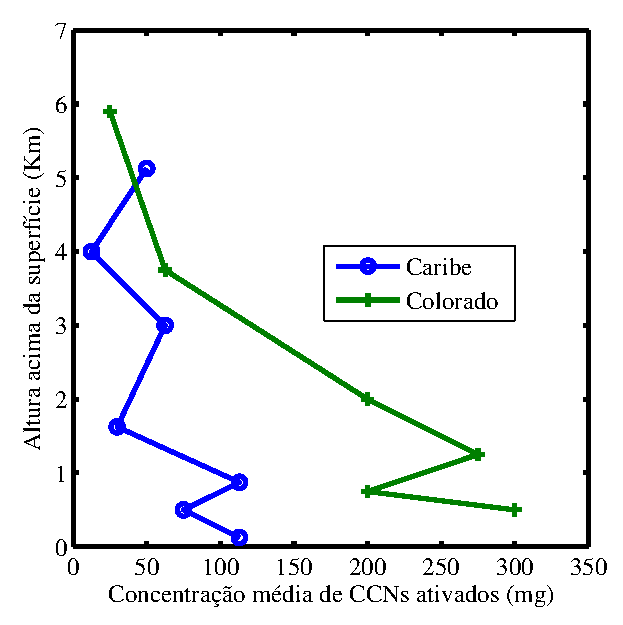
\includegraphics[scale=1.0]{eps/medidasAero2.eps}\\
\end{center}
\caption{\label{medidasAero}\hspace{-0.1em} concentra\c{c}\~{a}o m\'{e}dia, por mg de ar (1 cm$^3$ a 20$^o$C e 840mb), de CCNs ativados na supersatura\c{c}\~{a}o de 0,35\% em rela\c{c}\~{a}o a altitude.}
\end{figure}

%% ------------------------------------------------------------------------- %%
\section{Rela\c{c}\~{a}o entre CCN e Got\'{\i}culas de Nuvens}
Howell, em 1949 \cite{Howell}, realizou os primeiros c\'{a}lculos da forma\c{c}\~{a}o de uma popula\c{c}\~{a}o de got\'{\i}culas a partir de uma distribui\c{c}\~{a}o de CCNs, considerando-se a taxa de resfriamento uniforme e que a temperatura e press\~{a}o eram praticamente constantes durante a forma\c{c}\~{a}o de nuvens. Tamb\'{e}m considera que os CCN consistiam de aeross\'{o}is mar\'{\i}timos (n\'{u}cleos de cloreto de s\'{o}dio seco). As vari\'{a}veis utilizadas nos c\'{a}lculos foram: a umidade relativa (supersatura\c{c}\~{a}o), a massa dos n\'{u}cleos, o raio das got\'{\i}culas e o tempo (para uma velocidade vertical conhecida e para cima, e o tempo \'{e} proporcional a altura de ascens\~{a}o da parcela).

Alguns resultados obtidos por Howell s\~{a}o ilustrados na Figura \ref{howell} cujos eixos est\~{a}o em escala logar\'{\i}tmica. Observa-se nessa Figura que inicialmente as got\'{\i}culas (\'{a}gua condensada sobre os n\'{u}cleos) crescem lentamente e em paralelo com o aumento da supersatura\c{c}\~{a}o. Nessa fase, o tamanho das got\'{\i}culas (exceto alguns n\'{u}cleos grandes e no caso de alta taxa de resfriamento) est\'{a} pr\'{o}ximo ao valor de equil\'{\i}brio. Ap\'{o}s alcan\c{c}ar a m\'{a}xima supersatura\c{c}\~{a}o, o crescimento torna-se muito r\'{a}pido. Contudo, devido ao consumo de vapor de \'{a}gua que condensa sobre as gotas, a taxa de crescimento diminui lentamente, para se tornar um valor estacion\'{a}rio.

Os c\'{a}lculos realizados por Howell tamb\'{e}m indicam que os tamanhos das got\'{\i}culas ativadas convergem, com o tempo, para um valor comum, caracterizando assim o estreitamento do espectro de got\'{\i}culas. Para uma alta taxa de resfriamento, maiores supersatura\c{c}\~{o}es s\~{a}o criadas e consequentemente muitos CCN pequenos s\~{a}o ativados.
Essa rela\c{c}\~{a}o ainda foi confirmada por E. Freud e colaboradores \cite{freud} atrav\'{e}s de medi\c{c}\~{o}es \textit{in-situ} em nuvens convectivas.

\begin{figure}[!hbt]
\begin{center}
\includegraphics[scale=0.6]{eps/howell.eps}\\
\end{center}
\caption{\label{howell}\hspace{-0.1em} Crescimento de n\'{u}cleos de cloreto s\'{o}dio de massas diferentes em fun\c{c}\~{a}o do raio do n\'{u}cleo e da supersatura\c{c}\~{a}o.}
\end{figure}


H\'{a} atualmente um crescente interesse no estudo dos CCN. A causa \'{e} a influ\^{e}ncia destes n\'{u}cleos sobre a forma\c{c}\~{a}o, propriedades \'{o}ticas e radiativas das nuvens, e portanto, sobre a temperatura m\'{e}dia e outras caracter\'{\i}sticas clim\'{a}ticas da Terra. Twomey \cite{Twomey3} sugeriu que um aumento na concentra\c{c}\~{a}o de CCNs na atmosfera pode acarretar um aumento no albedo (raz\~{a}o entre a intensidade de fluxo refletido e o fluxo incidente) das nuvens via um aumento de cobertura. Como consequ\^{e}ncia pode haver um resfriamento no clima terrestre (efeito Twomey).

No ambiente continental estudos recentes indicam que altas concentra\c{c}\~{o}es de aeross\'{o}is, produzidos por queima de florestas, contribuem para a inibi\c{c}\~{a}o de chuvas na regi\~{a}o amaz\^{o}nica com a consequente mudan\c{c}a no ciclo hidrol\'{o}gico da regi\~{a}o \cite{Andreae,Debry}. Considerando-se o tamanho da regi\~{a}o amaz\^{o}nica, uma mudan\c{c}a no ciclo hidrol\'{o}gico certamente trar\'{a} importantes consequ\^{e}ncias econ\^{o}micas e sociais. Assim sendo, medir a concentra\c{c}\~{a}o de CCNs, mapear a sua origem e o seu destino final torna-se importante no contexto de mudan\c{c}as clim\'{a}ticas de larga escala.








